\thispagestyle{only-cfoot}
\section{Experiment setup}\label{s:ExperimentSetup}

% \todo{Write a chapter outline}

% Comparative experiment

% Agglomeration config, algorithm inputs ?

% leverage containerization to resource usage optimization -> 0.5cpu -> do porowniania wynikow schedulingu z optymalnym wykorzystaniem

This chapter describes in detail the experimental environment, its configuration, and setup process -- including the input for the algorithms run by the static scheduler.
The metrics used for evaluation are also introduced along with the reasons for their exploitation.

%%%%
\subsection{Environment}\label{s:ExperimentSetup:Environment}

% \todo{AWS, EKS, Eksctl i opis konfiguracja klastra}
As the prerequisites for this work indicate, the experiment was meant to be conducted in a computing cloud environment. % in Motivation section
To fulfill them, the AWS platform has been chosen as a target provider of resources to setup and deploy the Kubernetes cluster on.
This decision was based on both service popularity and our familiarity with it.

%

To setup the Kubernetes cluster in a cloud environment, the EKS (section \ref{s:ProblemDomain:EKS}) service was used.
The process has been further simplified by leveraging a \emph{eksctl} tool, which enabled the configuration of a cluster through a single file as shown in listing \ref{lst:ex-setup:eksctl-config}.
In the case of an experiment with larger workflow, to adjust the cluster computing capabilities, the number of nodes in each group configuration had been increased, which changed a vCPU count from 8 to 32 in total.


% \todo{obrazek, lub fragment konfiguracji + Hyperflow}
%%%%%%% Agglo Config 
\numberwithin{lstlisting}{section}
\smallskip
\begin{center}
\begin{minipage}{0.70\textwidth}
\lstset{
    basicstyle=\color{blue}\mdseries\fontsize{8}{9}\selectfont,
    moredelim=**[il][\color{black}\mdseries{:}\color{black}\mdseries]{:},
}
\centering
\begin{lstlisting}
apiVersion: eksctl.io/v1alpha5
kind: ClusterConfig

metadata:
  name: cluster-1
  region: us-east-1

availabilityZones: ["us-east-1d",  "us-east-1f"]

nodeGroups:
  - name: hyperflow-engine
    labels: { nodetype: hfmaster }
    instanceType: m5.xlarge
    desiredCapacity: 1
  - name: hyperflow-worker-1
    labels: { nodetype: worker1 }
    instanceType: m5.xlarge
    desiredCapacity: 1
  - name: hyperflow-worker-2
    labels: { nodetype: worker2 }
    instanceType: m5a.xlarge
    desiredCapacity: 1
\end{lstlisting}
\captionof{lstlisting}{Configuration for eksctl to setup cluster infrastrucutre}
\label{lst:ex-setup:eksctl-config}
\end{minipage}
\end{center}
%%%%%%%


All experiments had been conducted in heterogeneous environments.
The heterogeneity was introduced by including two separate node groups in a cluster, where each of them comprises of different machine instances.
Their detailed specifications are presented in the table \cref{tab:ex-setup:instances}.
This was decided to obtain more natural results from the experiments, as the scheduling algorithms are native to such environments.


\begin{table}[H]
    \centering
    \begin{tabular}{|c|c|c|c|c|c|}
    \cline{1-5}
        \multirow{2}{*}{Instance name} 
        &
        \multirow{2}{*}{vCPUs}
        &
        \multirow{2}{*}{Memory}
        &
        \multicolumn{2}{|c|}{Specification details} \\
    \cline{4-5}
        & & & CPU Type & CPU Clock \\
    \cline{1-5}
        m5.xlarge & 4 & 16 GiB & Intel Xeon Platinum 8175M & 2.50 GHz \\
    \cline{1-5}
        m5a.xlarge & 4 & 16 GiB & AMD EPYC 7571 & 2.55 GHz \\
    \cline{1-5}
    \end{tabular}
    \caption{Instance specifications for machines forming the cluster}
    \label{tab:ex-setup:instances}
\end{table}


Containerization is a quite flexible method of virtualization regarding resource allocation.
It allows fractions of a specific resource in a pool to be assigned and utilized by a single container.   
As the HEFT and PEFT algorithms assume that each task is being executed on a separate processing unit, a static configuration was provided for a resource request for pod creation.
To unify the resource assignment values across different experiment scenarios, the setup was unified as following:

\begin{itemize}[topsep=0pt]
  \item{
\emph{CPU request} was set to 0.85, ensuring there were no more containers than the vCPU on the given node
};
  \item{
\emph{MEM request} was increased to 1GiB, to mitigate possible unexpected issues with high memory usages coming from request limitations.
}
\end{itemize}
% lista requestow CPU request, MEM request
The results achieved with such a configuration were juxtaposed with results from an \emph{utilization-based} experiment scenario.
To set the optimal resource requests, separate experiments were run to  measure the task execution times for each available type of machine instance.
Usages were first averaged for each task in a workflow and then for each operation the task was associated with.
Then, during the workflow execution, the CPU requests were set to the extracted values, representing an expected optimal resource usage, respectively, for each operation.
The values used in this configuration are listed in section \ref{s:Evaluation:ResourceOptimal} along with the results.

% \begin{table}[H]
%     \centering
%     \begin{tabular}{|c|c|c|c|c|c|}
%     \cline{1-6}
%         \multirow{2}{*}{Instance name} 
%         &
%         \multicolumn{5}{|c|}{Metrics} \\
%     \cline{2-6}
%         & Makespan & Job slowdown & SLR & CO & Critical CO \\
%     \cline{1-6}
%         m5.xlarge & x & x & x & x & x \\
%     \cline{1-6}
%         m5a.xlarge & x & x & x & x & x \\
%     \cline{1-6}
%     \end{tabular}
%     \caption{Instance specifications of machines forming the cluster}
%     \label{tab:ex-setup:optimal-usages}
% \end{table}




%%%%
\subsection{Scheduler plugin input}\label{s:ExperimentSetup:Input}

% \todo{Opisać input algorytmów schedulingu, jak zostały wyznaczone wartości, zaprezentować same plany wykonania po wykonaniach algorytmów}

% \todo{dopisz tytulem wstepu ze korzystamy z pluginu - hetf i peft}

The scheduling solution presented in this work creates a plan of workflow execution with either HEFT or PEFT scheduling algorithms. 
Data required for input by both algorithms used in the scheduler has the same format.
It comprises of two matrices, one filled with computation costs and another with communication costs.
The costs of computation have to be provided separately for each task and each processing unit in the cluster.
As for communication costs, they need to be provided for each pair of processors.

In the conducted experiments, a few assumptions were made during the input matrix composition.
The execution time for each task, excluding the time overhead spent on containerization, was taken as a task computation cost.
As the cluster is composed of nodes with only two possible different instance types, it also has been assumed that the task execution times should be the same for each processor within a single node group.
Thus, only two execution times were provided for every task, one for each node group in the cluster:

% \medskip
% \begin{minipage}{0.65\textwidth}
% {\footnotesize Depicts Kubernetescluster components and processes distributed among them.\par}
% \end{minipage}
\begin{align}
C_{comp}=
\begin{bmatrix}
T_{0, 0} & T_{0, 1} & \dots & T_{0, j}\\
T_{1, 0} & \ddots &  & \\
\vdots &  & \ddots & \\
T_{i, 0} &  &  & T_{i, j}\\
\end{bmatrix}.
\end{align}

\begin{center}
\medskip
\begin{minipage}{0.5\textwidth}
% \centering
\small
$C_{comp}$ -- computation cost matrix

$T_{i, j}$ -- time to execute \emph{i-th} task on \emph{j-th} processor
\end{minipage}
\medskip
\end{center}
% \begin{bmatrix}
% 1 & 2 & 3\\
% a & b & c
% \end{bmatrix}
As all cluster nodes are located within a single network managed within a single data centre, it was assumed that the communication cost should be the same for each processor pair.
The only exception was the communication of a processing unit with itself, which was assumed to have no cost:


\begin{align}
C_{comm}=
\begin{bmatrix}
0 & 1 & \dots & 1\\
1 & \ddots &  & \vdots \\
\vdots &  & \ddots & 1 \\
1 & \dots & 1 & 0 \\
\end{bmatrix}.
\end{align}

\begin{center}
\medskip
\begin{minipage}{0.6\textwidth}
\small
$C_{comm}$ -- communication cost matrix form experiment setup
\end{minipage}
\medskip
\end{center}

% In conducted experiments we set all the values

% \todo{Dodaj obrazki planow wykonania workflow 3x HEFTT i PEFT}

%%%%%
\begin{figure}[H]
\begin{subfigure}{1.0\textwidth}
\centering
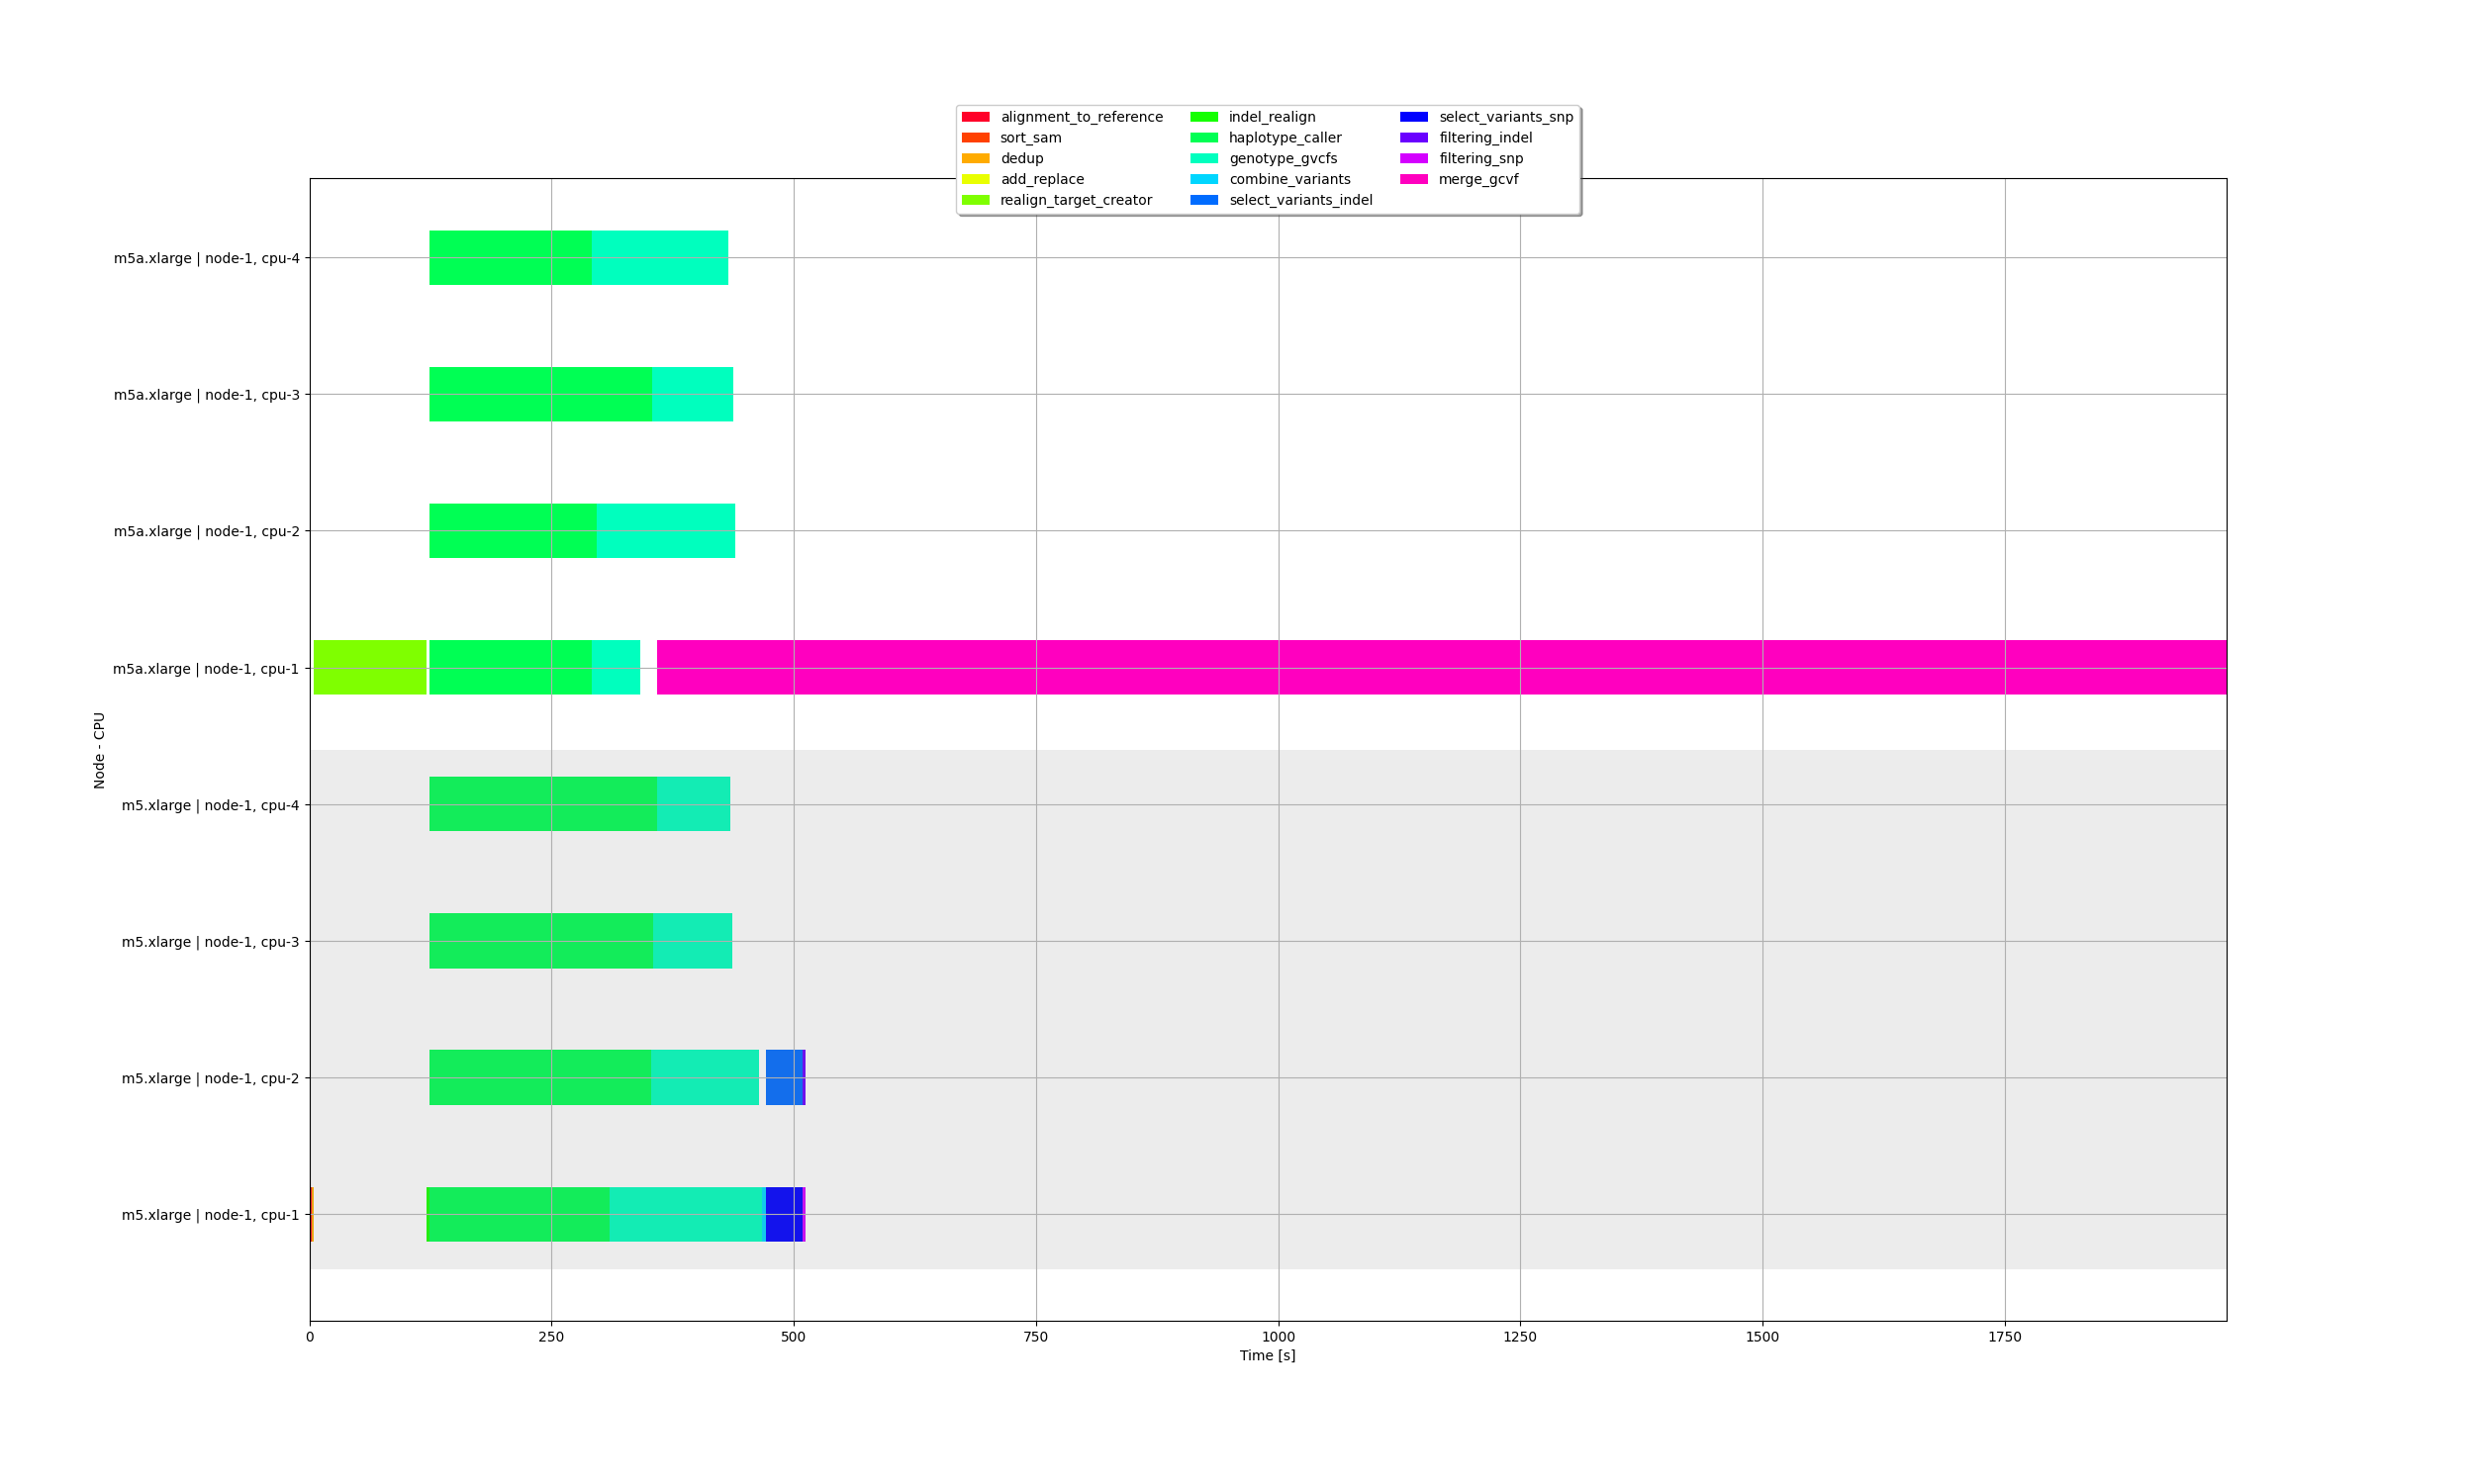
\includegraphics[width=1\linewidth]{figures/5-2-soykb_heft.png}
\caption[Schedules computed for SoyKB workflow - HEFT]{HEFT}
\label{fig:setup-input:soykb:heft}
\end{subfigure}
\begin{subfigure}{1.0\textwidth}
\centering
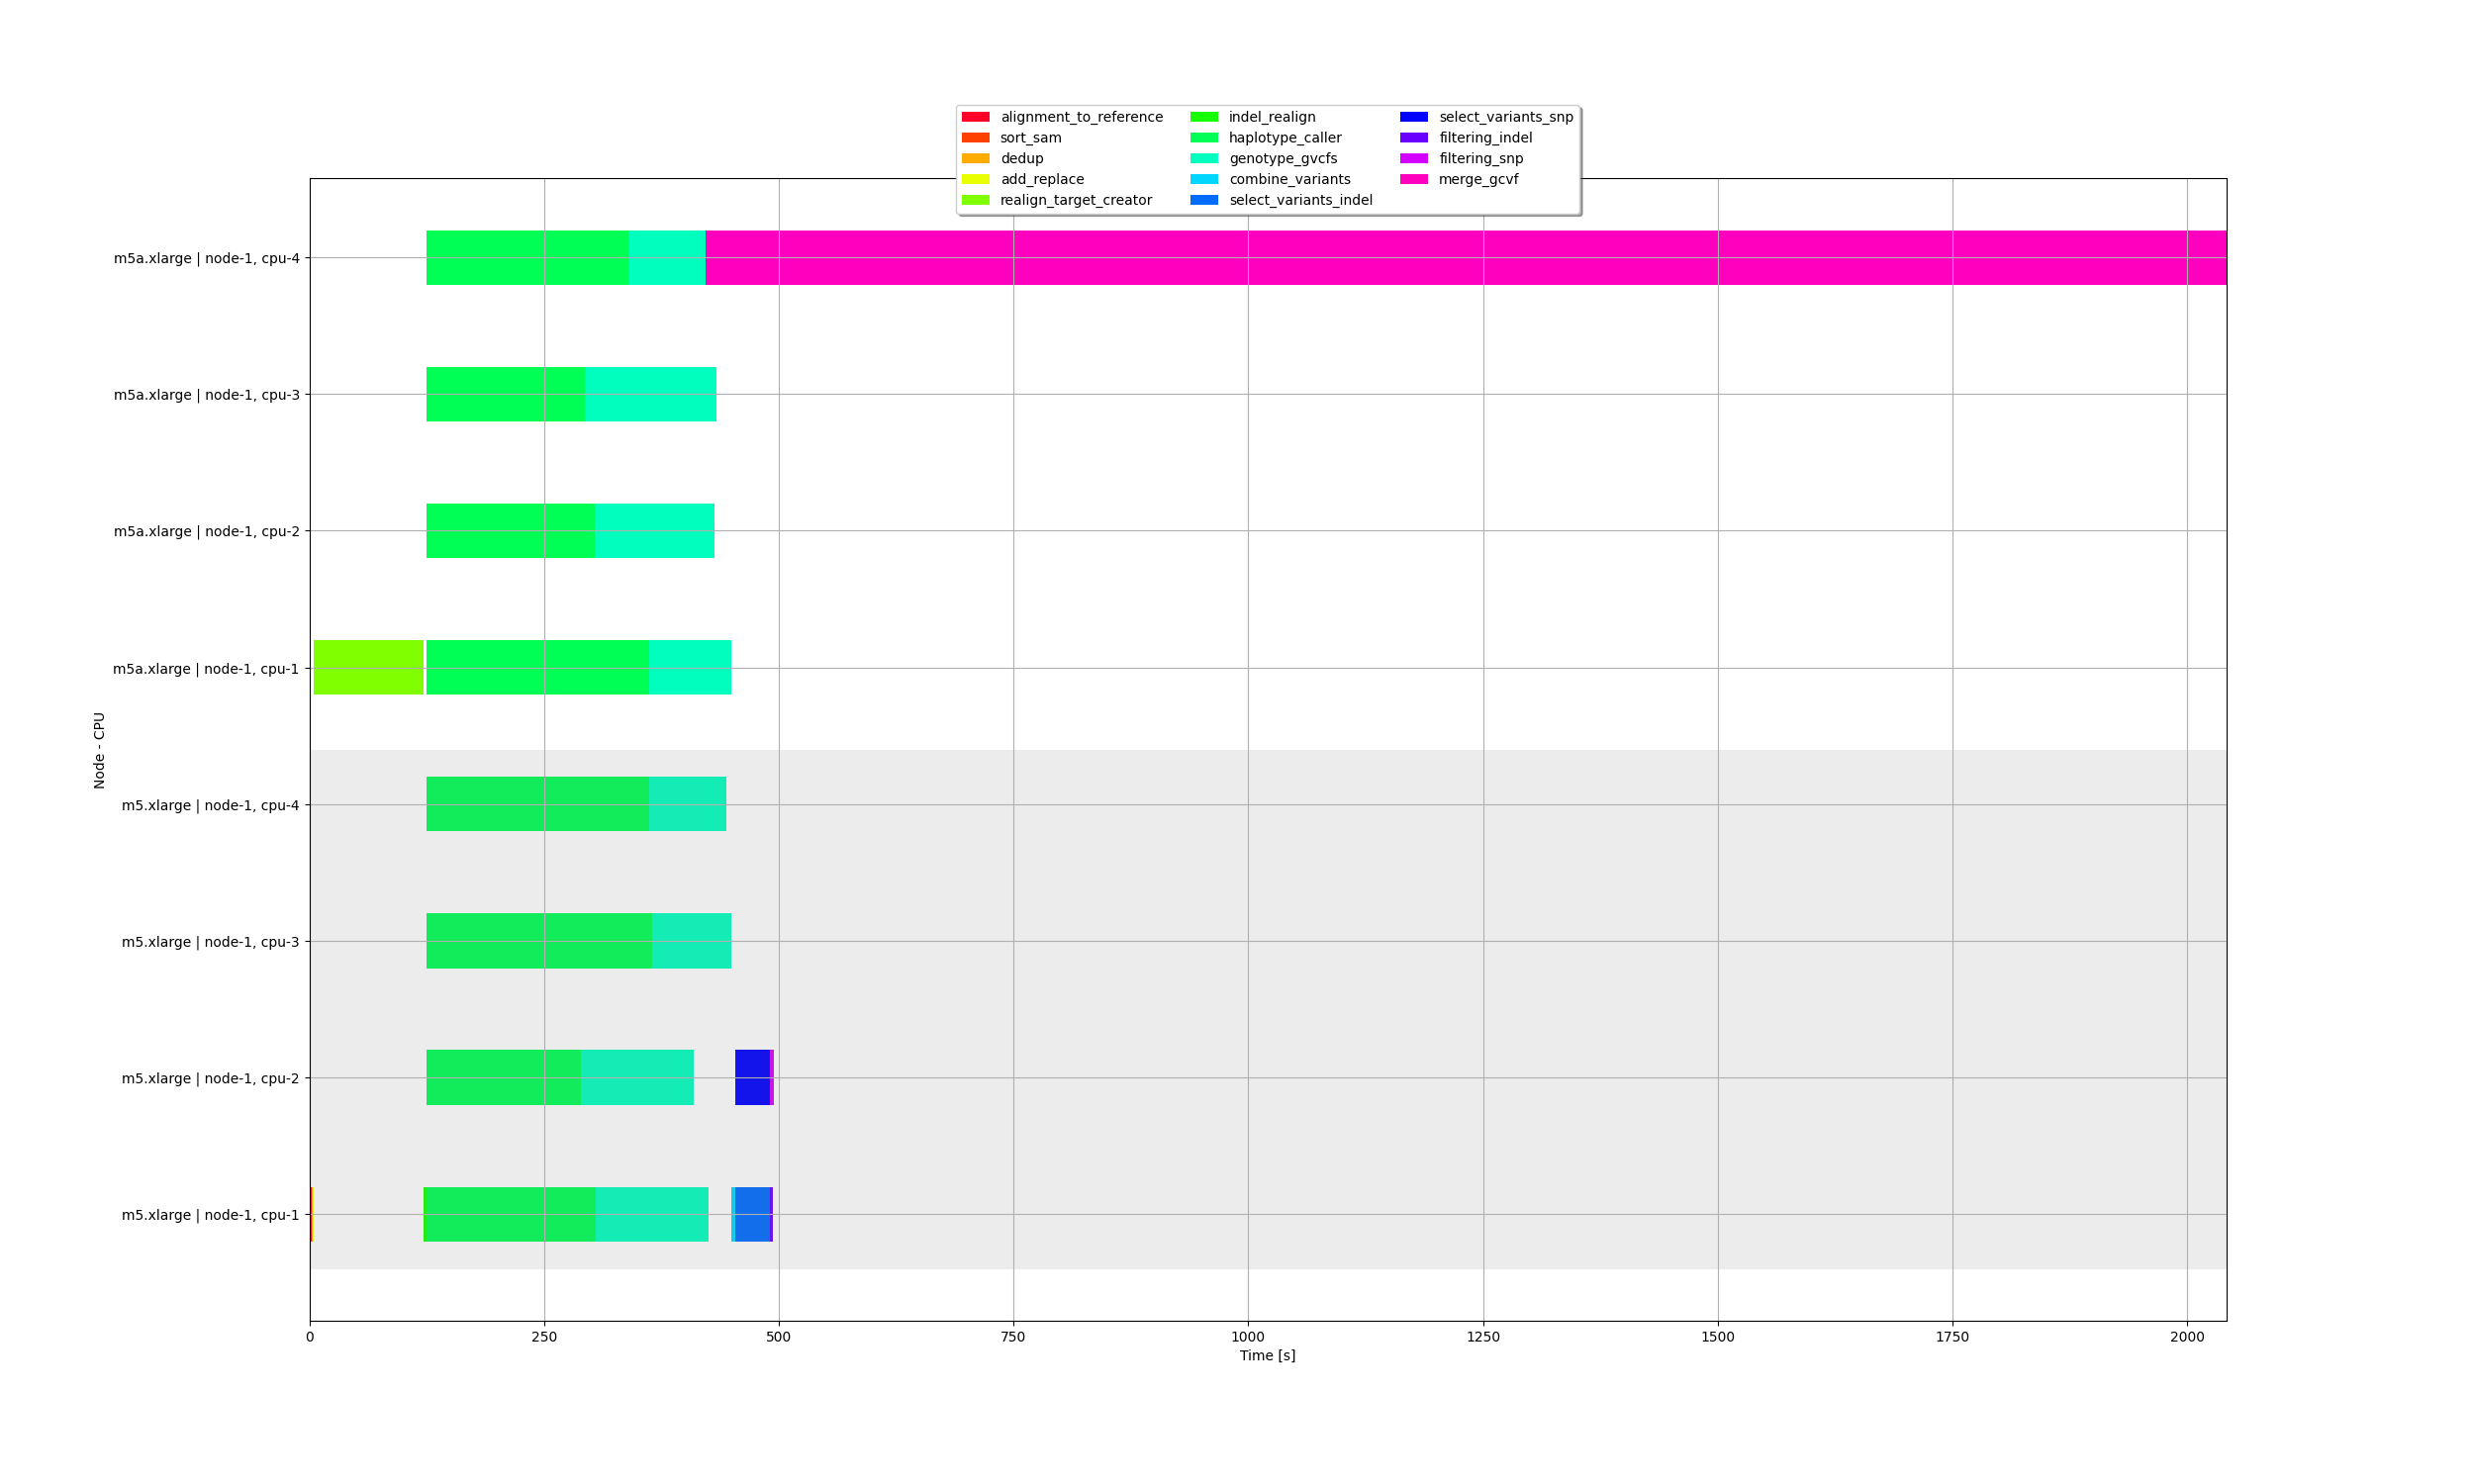
\includegraphics[width=1\linewidth]{figures/5-2-soykb_peft.png}
\caption[Schedules computed for SoyKB workflow - PEFT]{PEFT}
\label{fig:setup-input:soykb:peft}
\end{subfigure}
\centering
%%
\caption[Schedules computed for SoyKB workflow]{Schedules computed for SoyKB workflow}
\label{fig:setup-input:soykb}
\end{figure}
%%%%%

%%%%%
\begin{figure}[H]
\begin{subfigure}{1.0\textwidth}
\centering
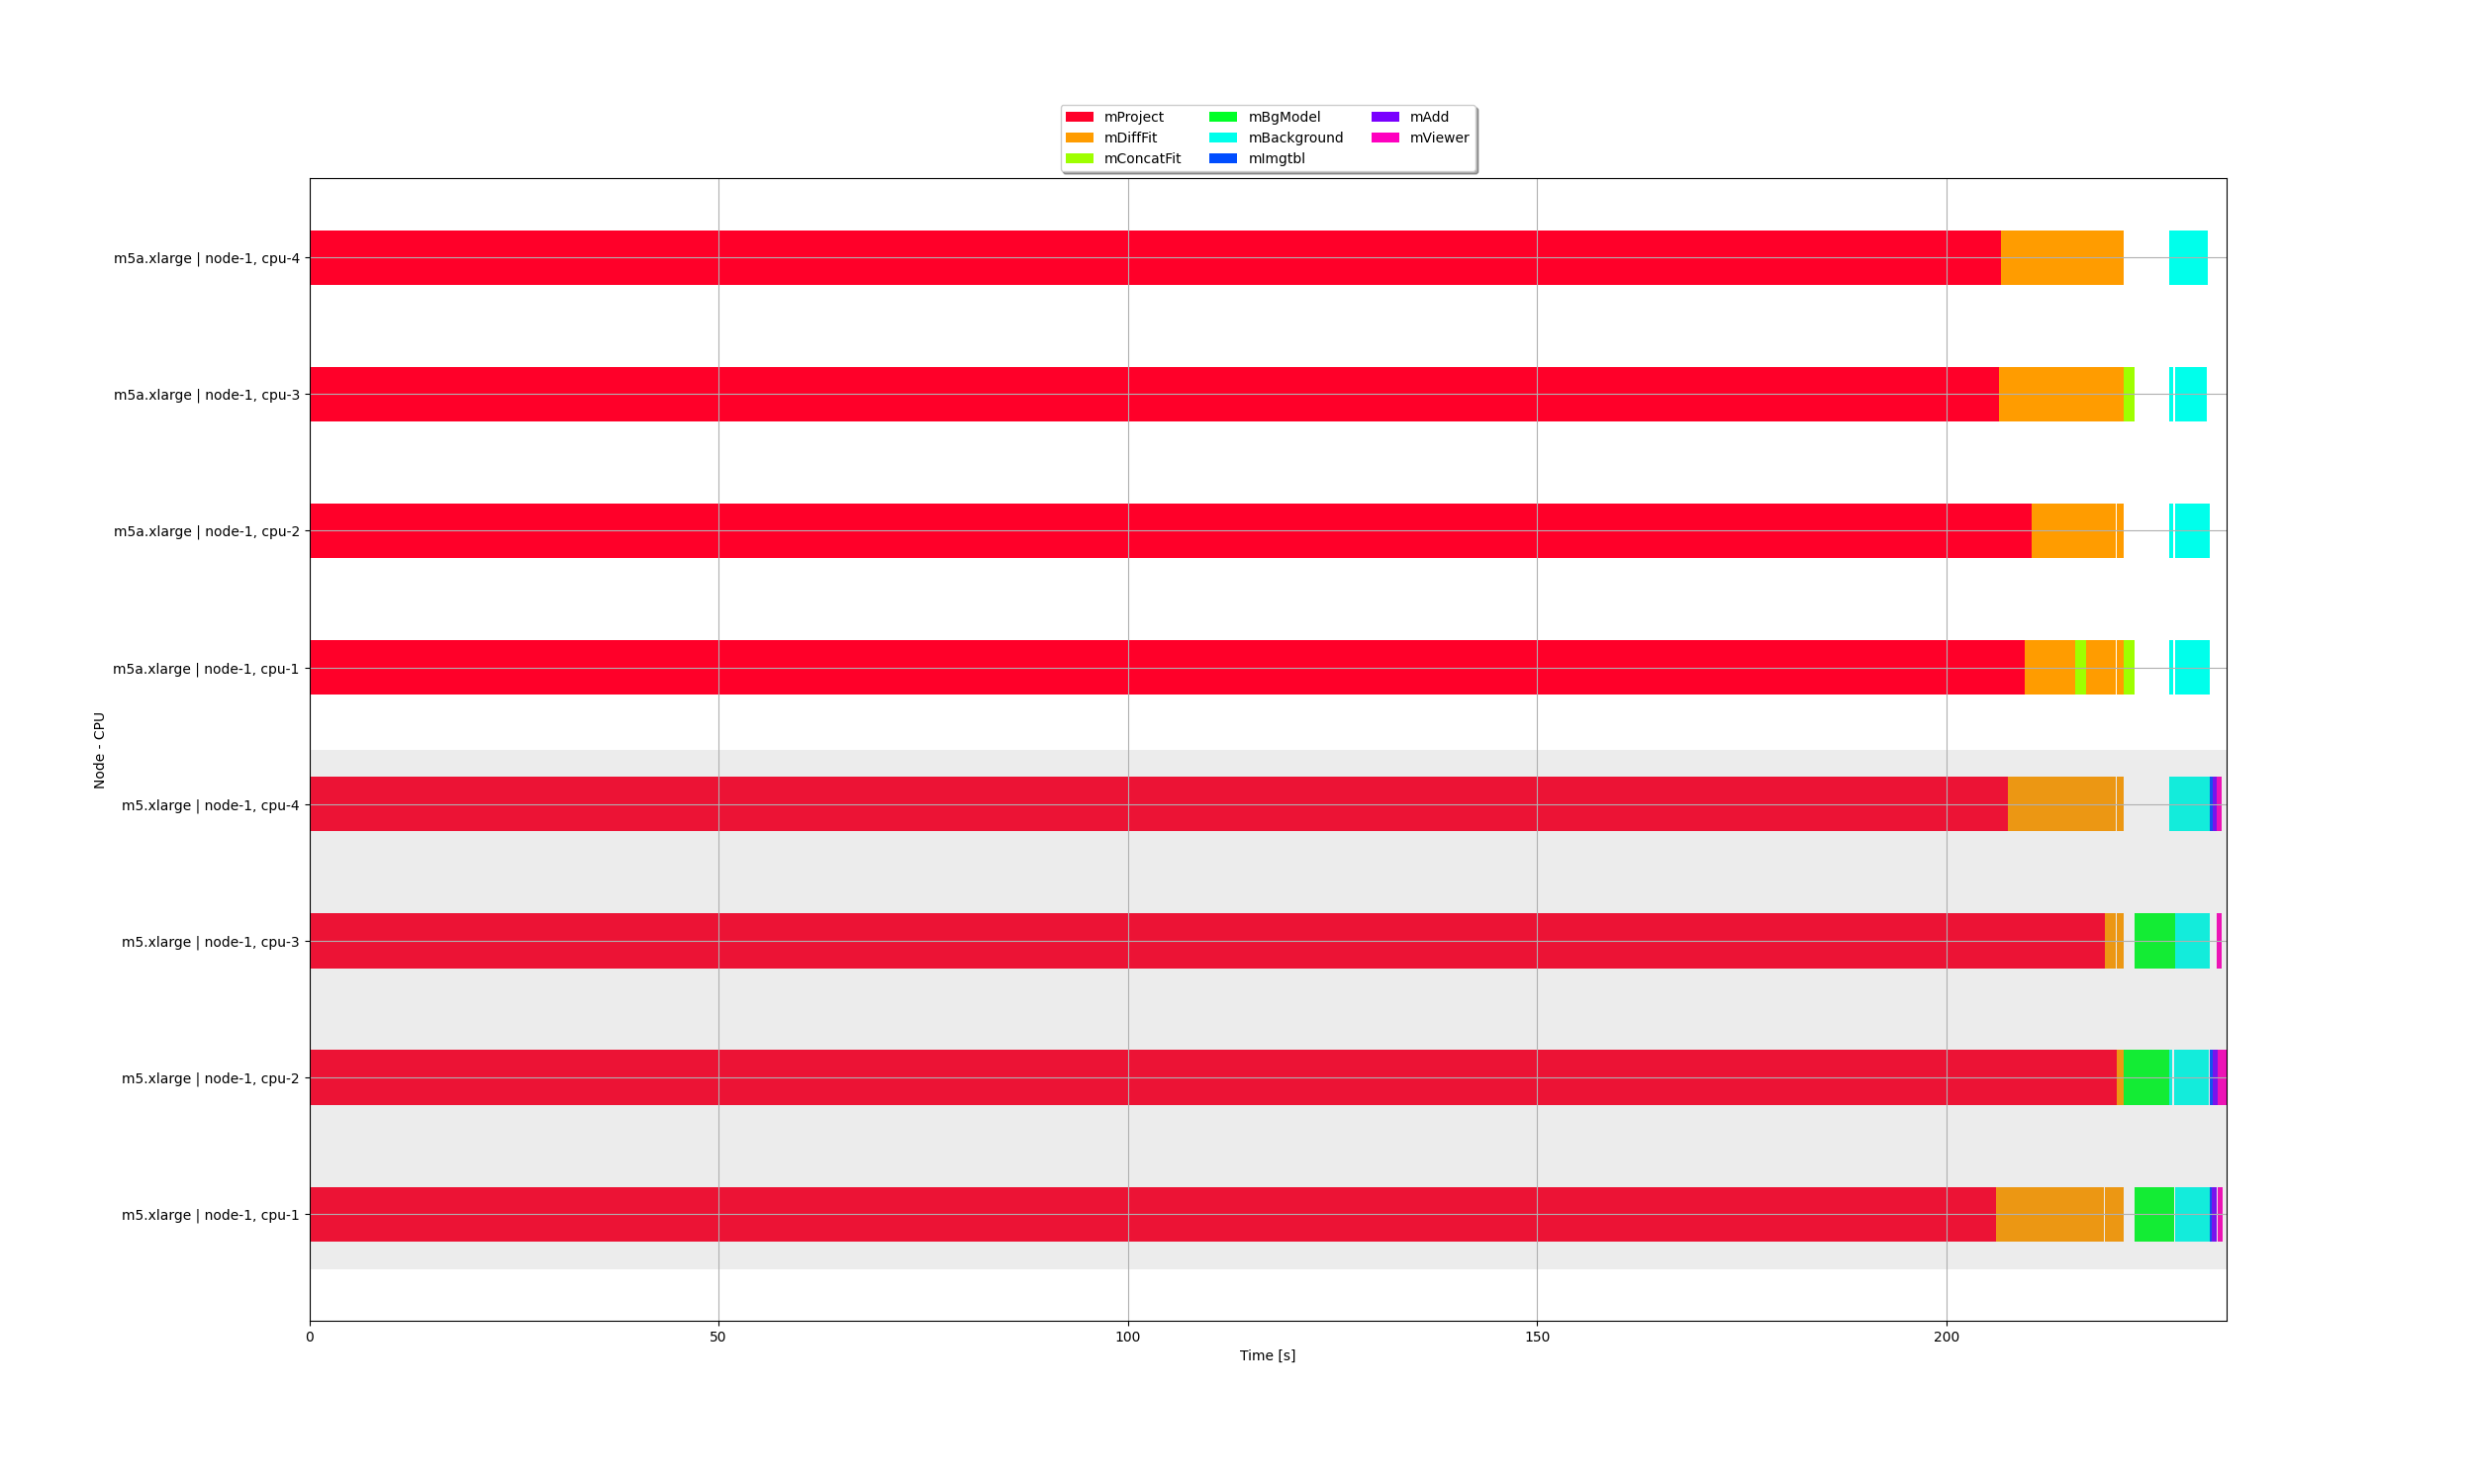
\includegraphics[width=1\linewidth]{figures/5-2-montage025_heft.png}
\caption[Schedules computed for Montage2-v0.25 workflow - HEFT]{HEFT}
\label{fig:setup-input:m025:heft}
\end{subfigure}
\begin{subfigure}{1.0\textwidth}
\centering
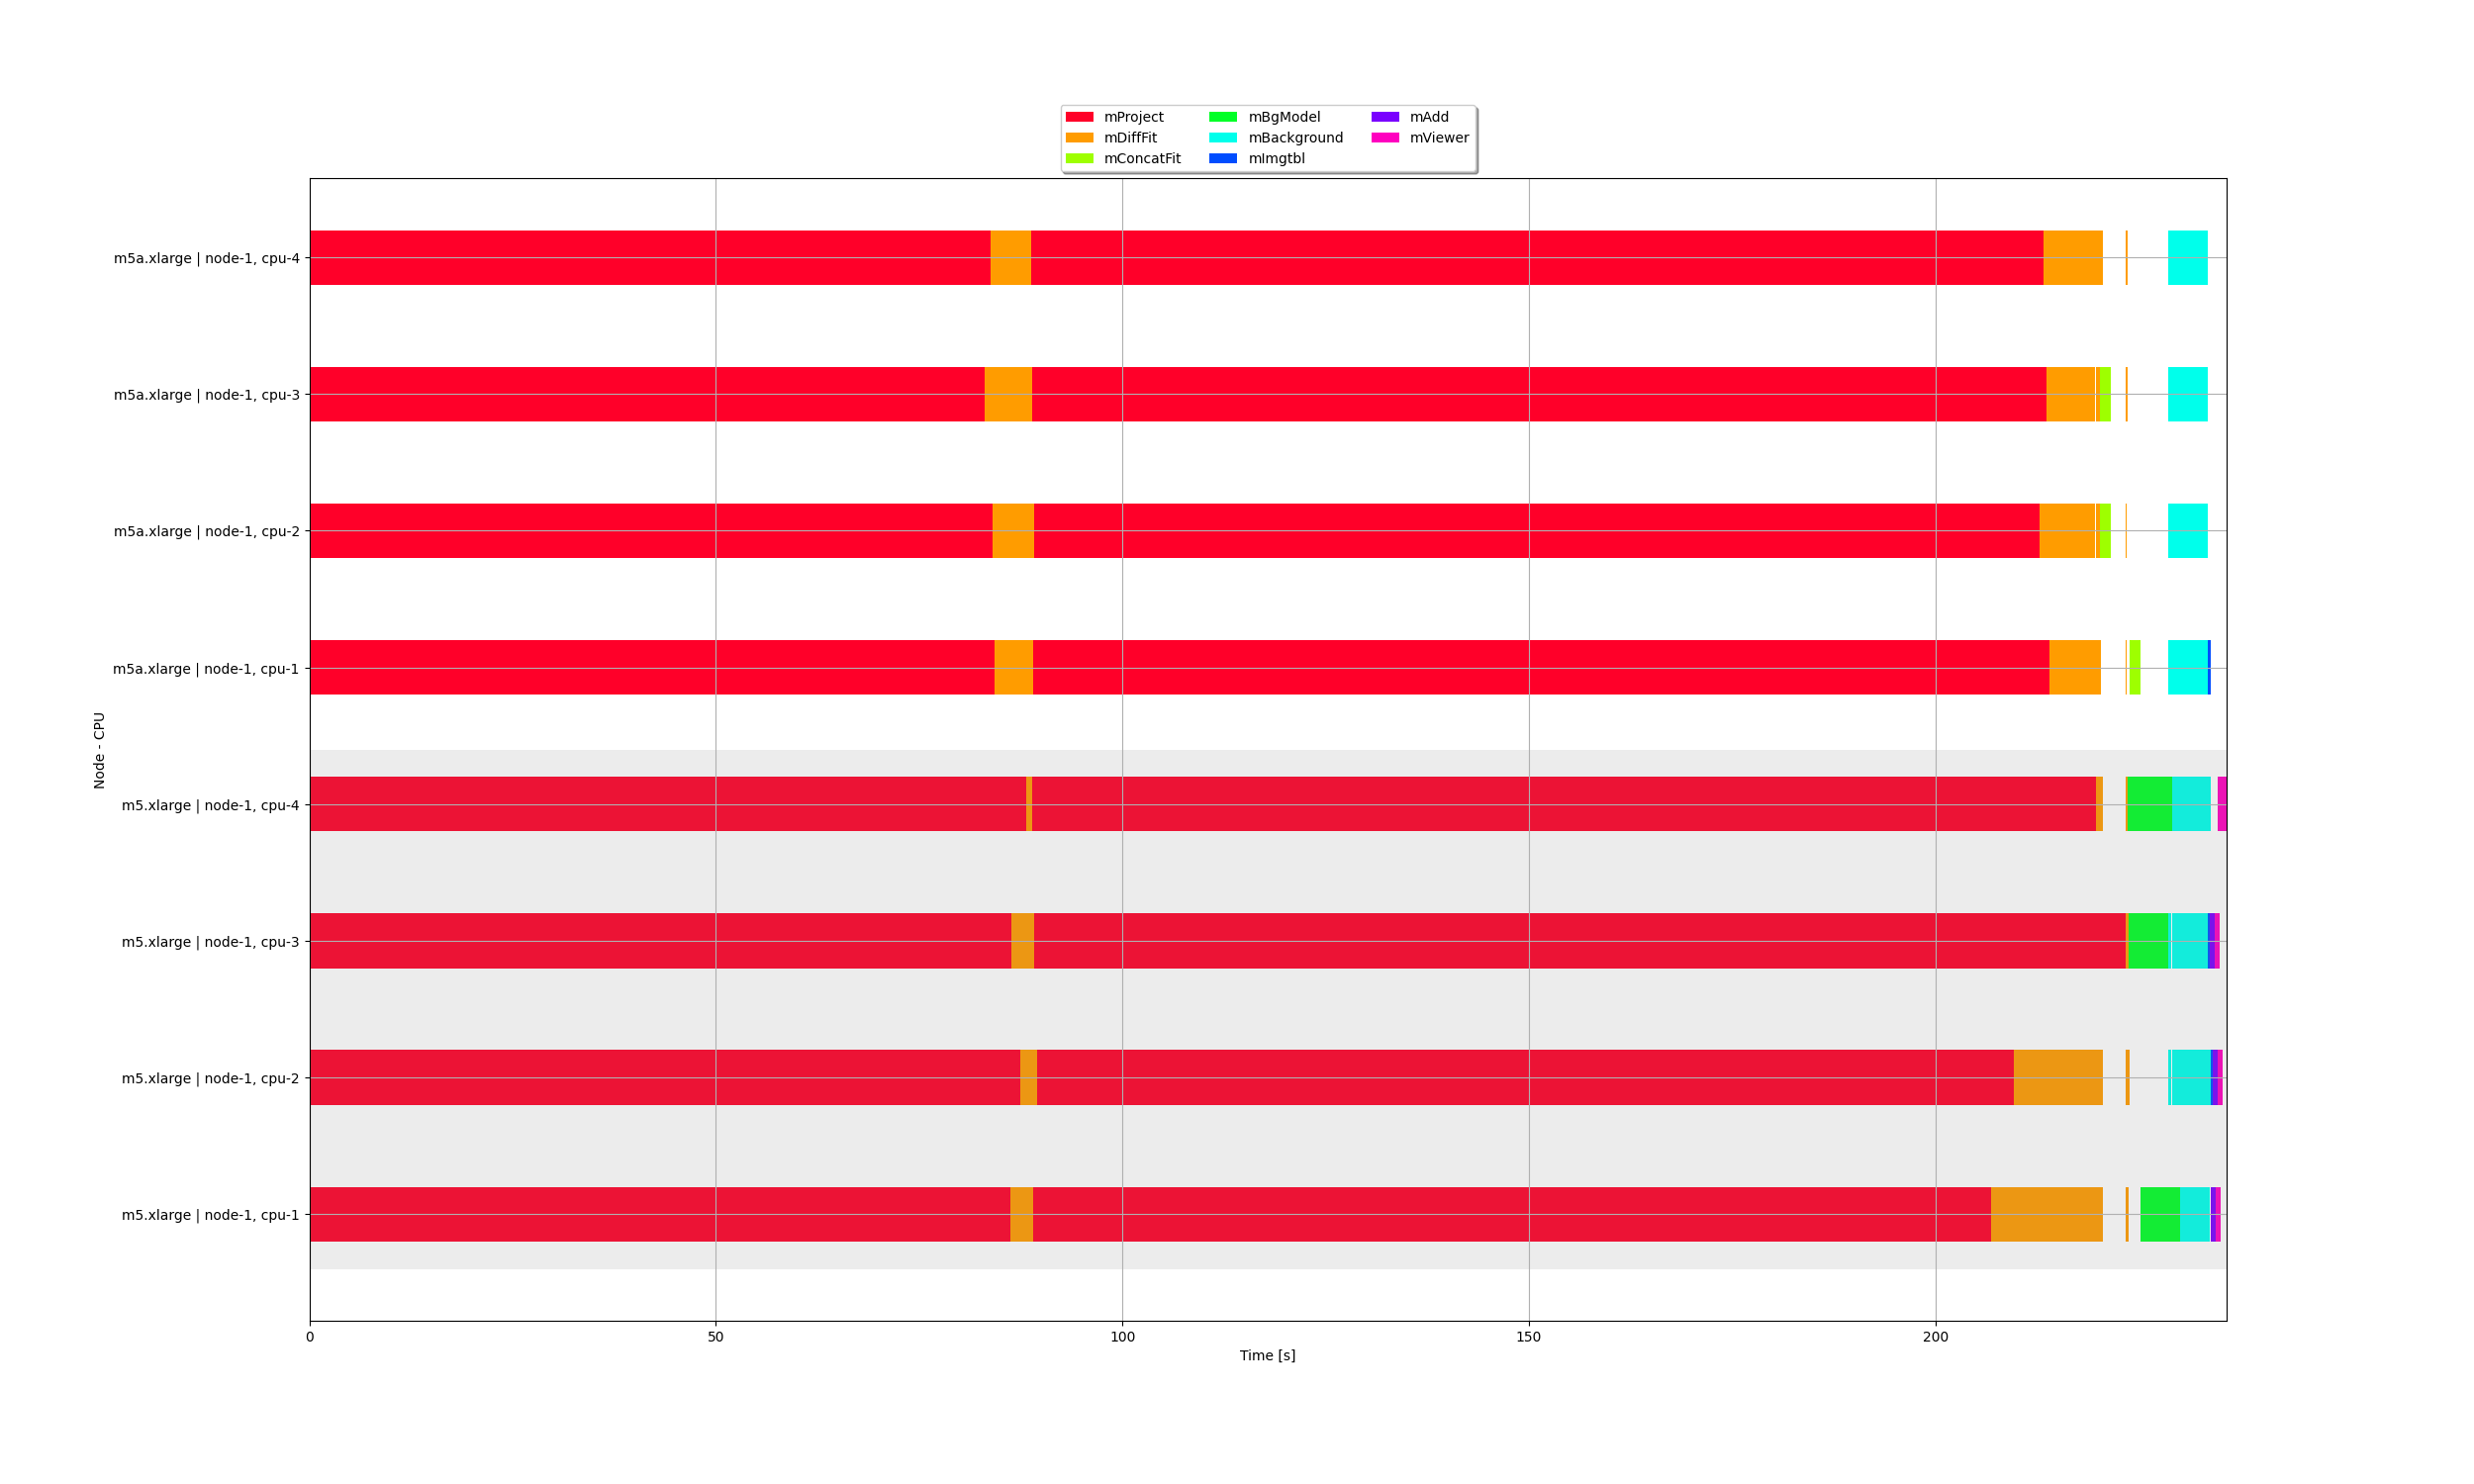
\includegraphics[width=1\linewidth]{figures/5-2-montage025_peft.png}
\caption[Schedules computed for Montage2-v0.25 workflow - PEFT]{PEFT}
\label{fig:setup-input:m025:peft}
\end{subfigure}
\centering
%%
\caption[Schedules computed for Montage2-v0.25 workflow]{Schedules computed for Montage2-v0.25 workflow}
\label{fig:setup-input:m025}
\end{figure}
%%%%%

%%%%%
\begin{figure}[H]
\begin{subfigure}{1.0\textwidth}
\centering
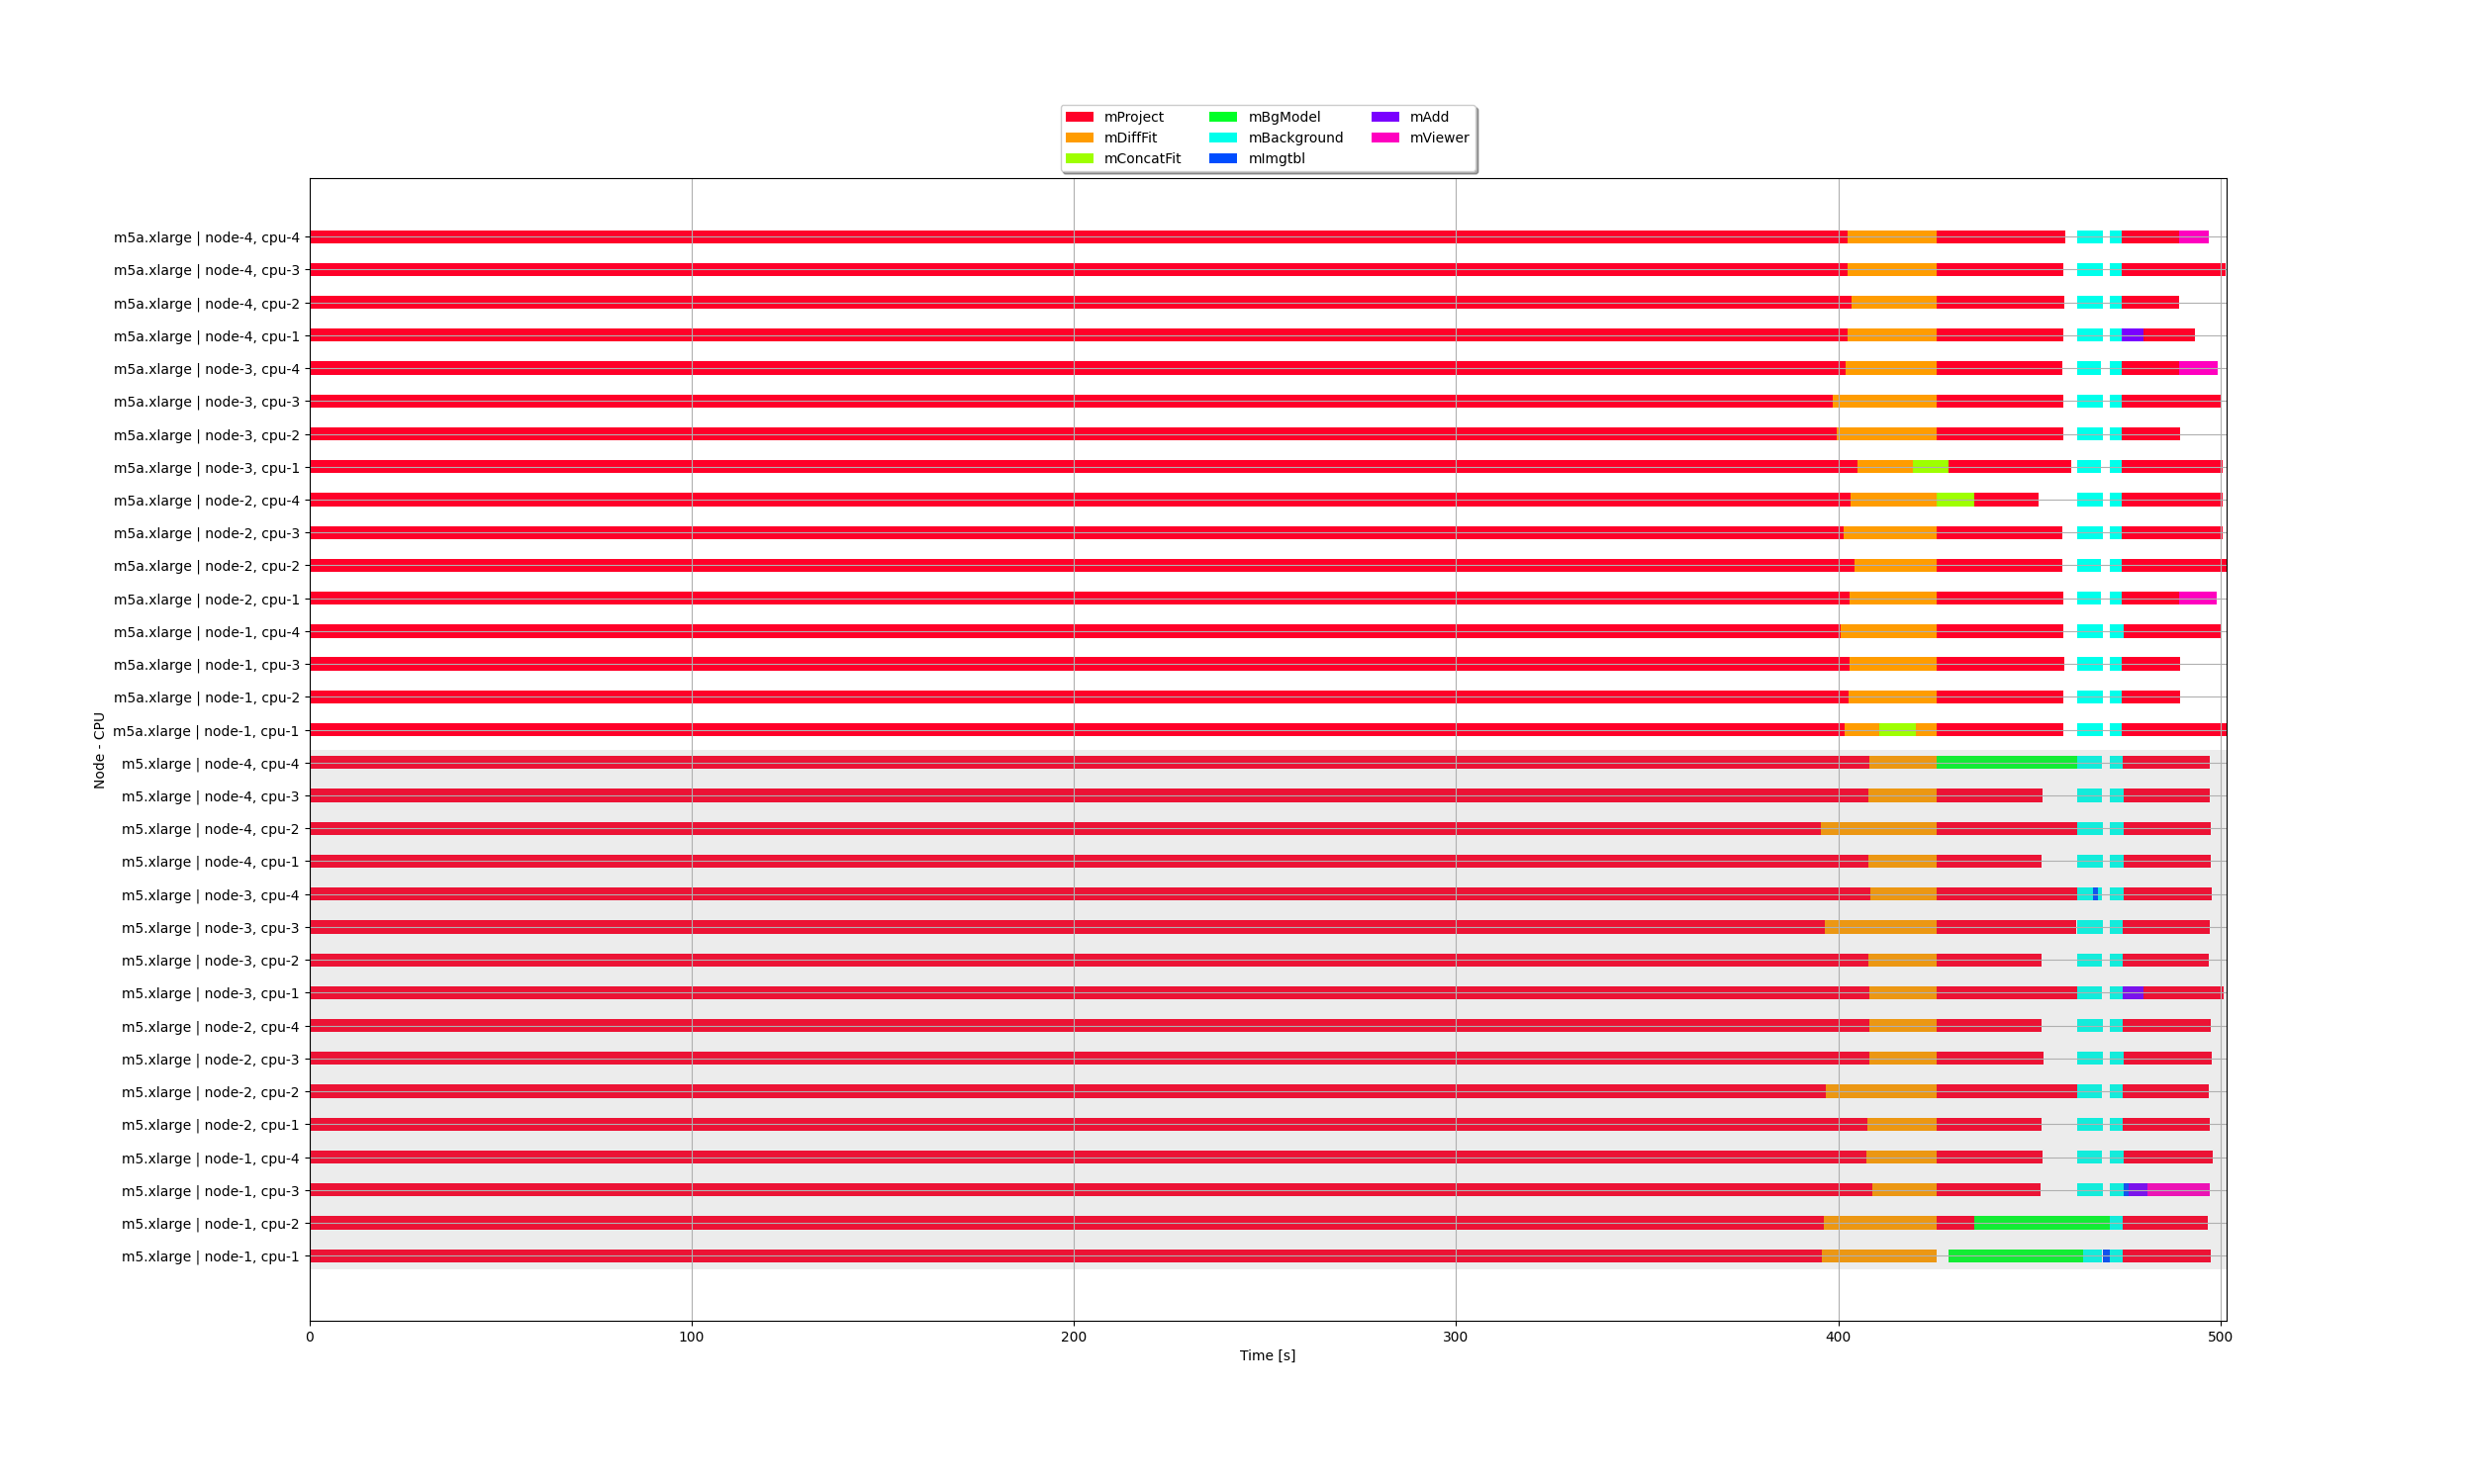
\includegraphics[width=1\linewidth]{figures/5-2-montage10_heft.png}
\caption[Schedules computed for Montage2-v1.0 workflow - HEFT]{HEFT}
\label{fig:setup-input:m10:heft}
\end{subfigure}
\begin{subfigure}{1.0\textwidth}
\centering
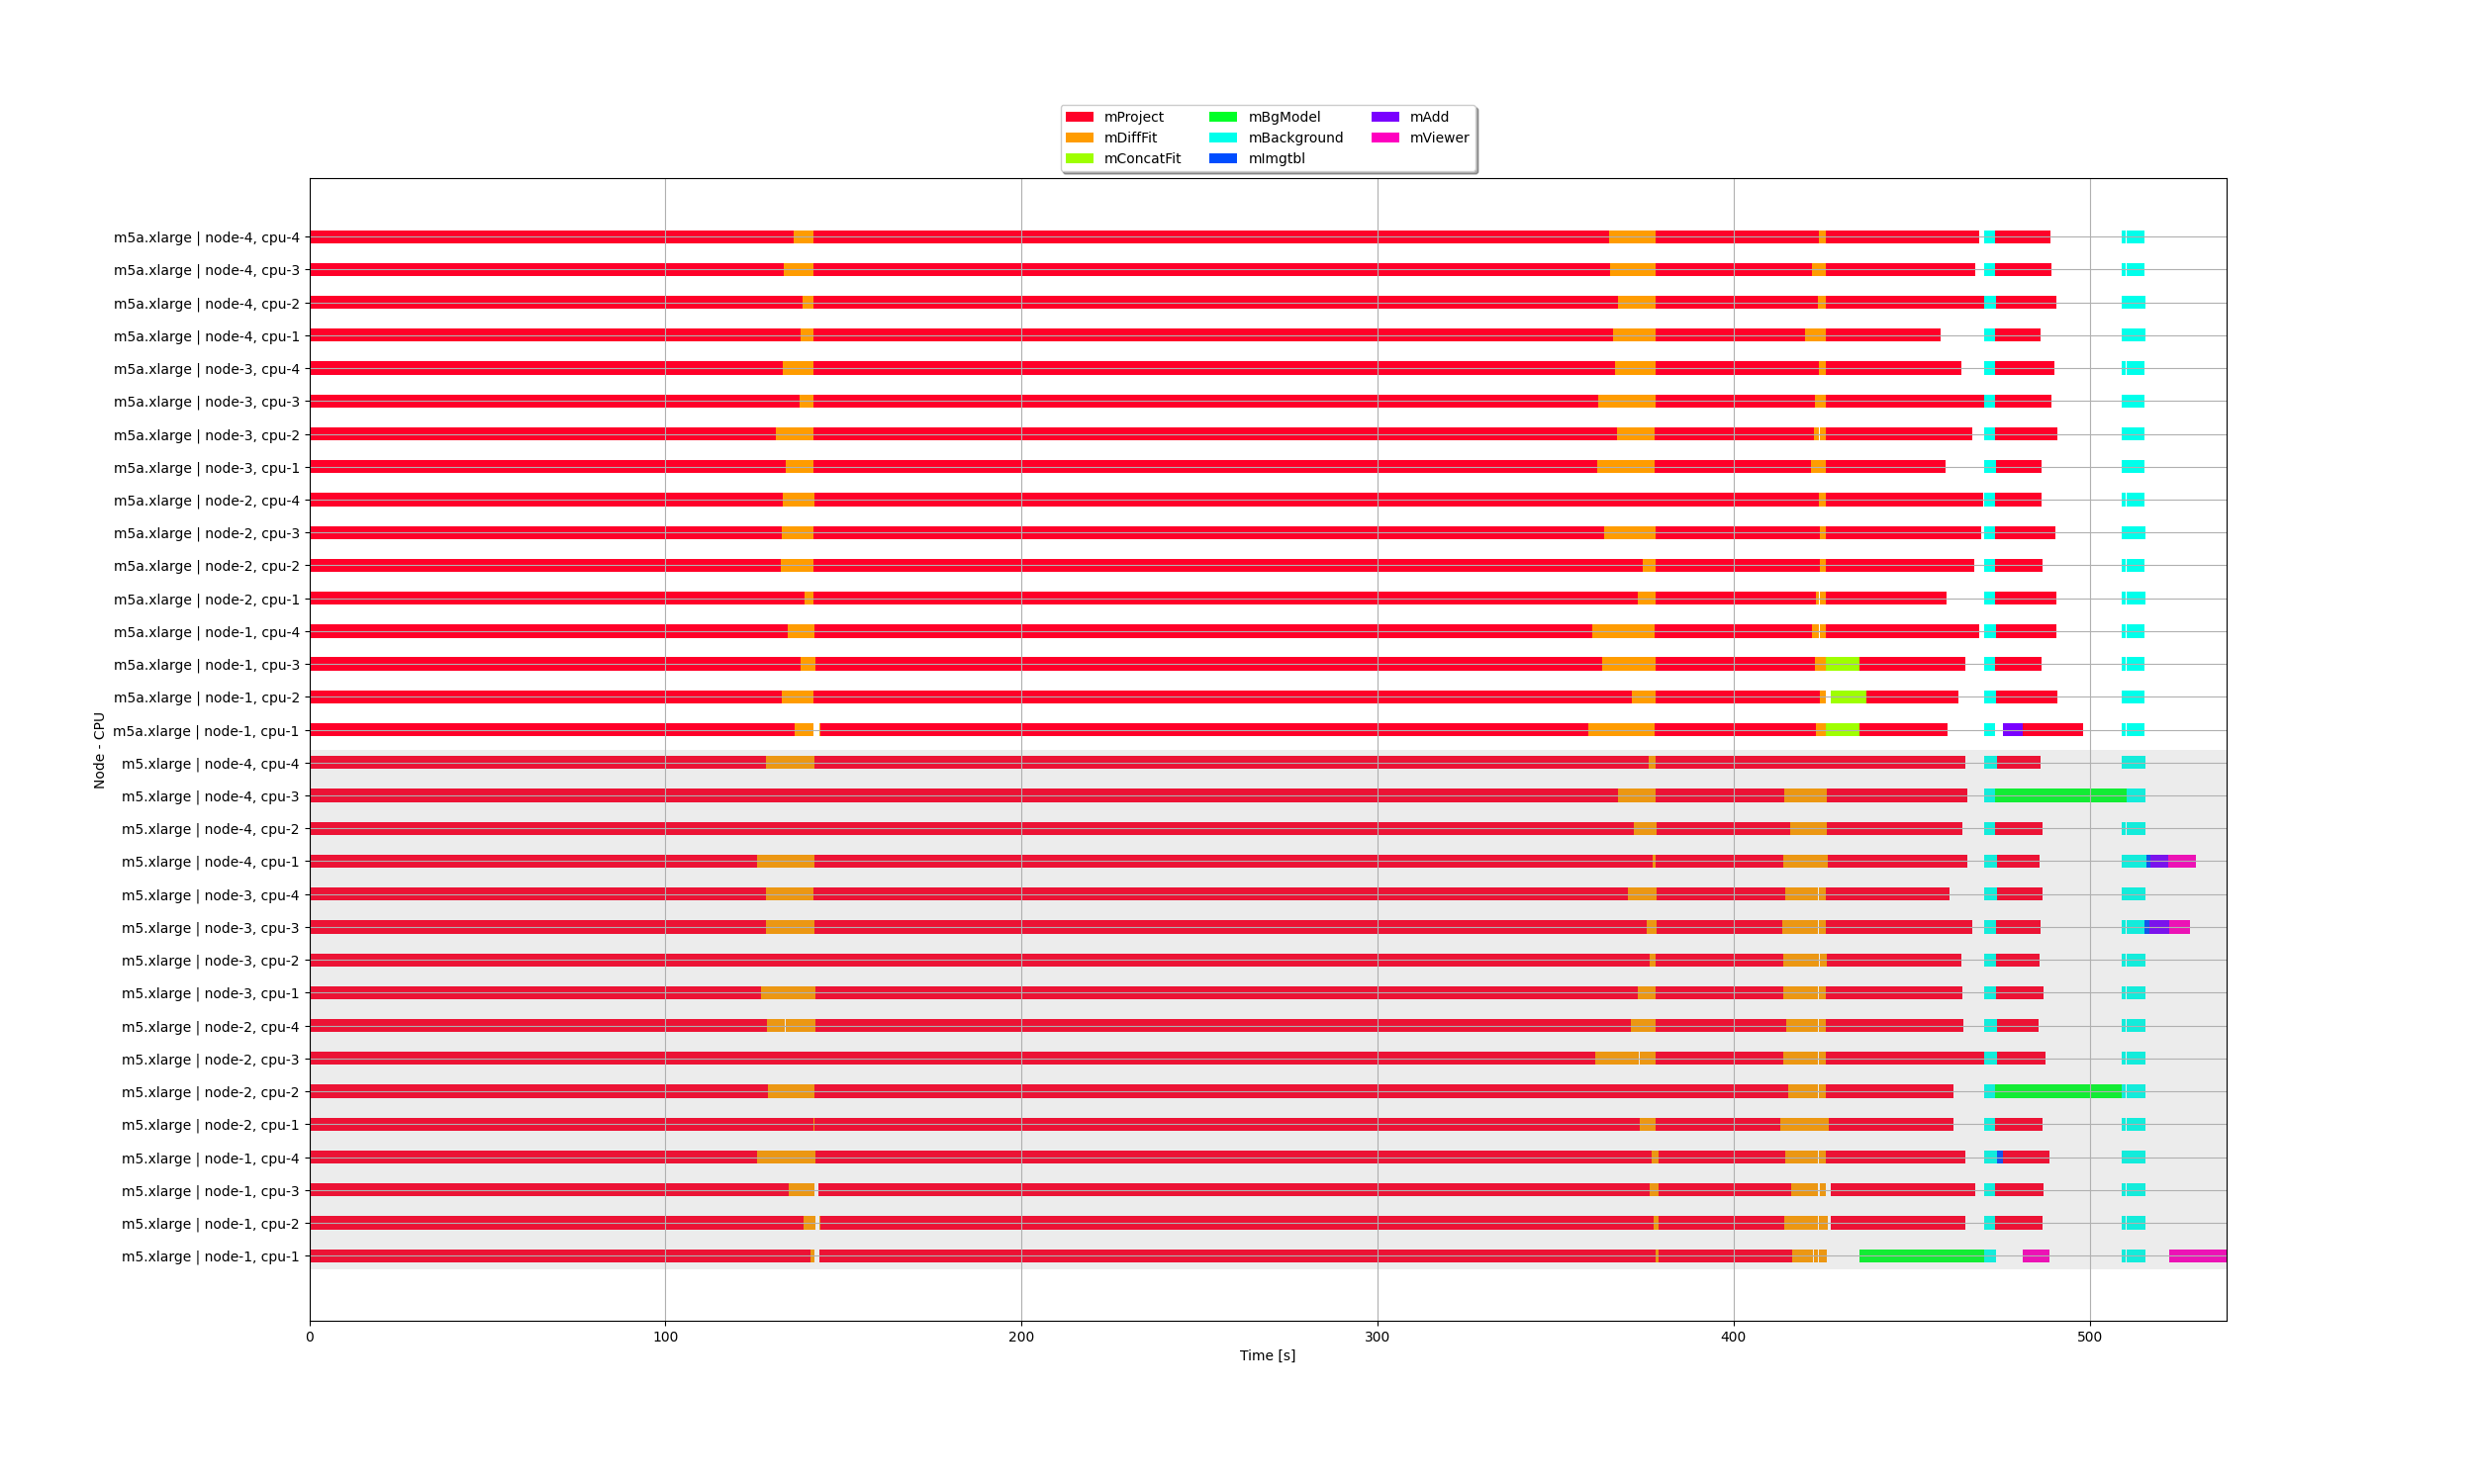
\includegraphics[width=1\linewidth]{figures/5-2-montage10_peft.png}
\caption[Schedules computed for Montage2-v1.0 workflow - PEFT]{PEFT}
\label{fig:setup-input:m10:peft}
\end{subfigure}
\centering
%%
\caption[Schedules computed for Montage2-v1.0 workflow]{Schedules computed for Montage2-v1.0 workflow}
\label{fig:setup-input:m10}
\end{figure}
%%%%%




%%%%
\subsection{Metrics}\label{s:ExperimentSetup:Metrics}

% \todo{opisać dokładniej wykorzystane metryki, załączyć wzory}

% list and explain all available operators T_arrival etc.
To evaluate and compare the performance of the applied scheduling approaches, four metrics were selected.
Each of them offers an insight on some aspect of the evaluated solution and allows analysis from different perspectives.
The data used for metric calculation comes from experiment logs and mostly consists of the resource usage values and timestamps for various events fired for each task in the workflow.

% \todo{Wyniki wyliczone skryptem XYZ i znajduja sie pod URL...}

\begin{center}
\medskip
\begin{minipage}{0.8\textwidth}
% \small
$J $ -- a set of jobs that belong to the given workflow \\
\smallskip
$CP$ -- a set of jobs that form a \emph{Critical Path} in a workflow graph \\
\smallskip
$W_{start}, W_{finish}$ -- times of a workflow start and finish, respectively \\
\smallskip
$T_{start}^j, T_{finish}^j$ -- times of a \emph{j} job start and finish, respectively \\
\smallskip
$T_{arrival}^j$ -- time when a \emph{j} job becomes executable, but is not yet scheduled \\
\smallskip
$T_{exec}^j$ -- execution time of a \emph{j} job, excluding containerization.

\end{minipage}
\medskip
\end{center}



The first metric, \emph{Makespan}, is one of the most common and most relevant representations of workflow execution performance.
It shows how much time, in seconds, is needed to complete all workflow tasks from the time it has started:

\begin{align}
Makespan = W_{finish} - W_{start}
.
\end{align}


Another metric used in the evaluation is \emph{Slowdown}.
Slowdown provides an insight on the scheduling strategy used in a selected approach, whether the execution of freshly available tasks or longer waiting ones is preferred.
The lower the slowdown ratio, the better response times of jobs across the application.
It is calculated for each job, however, since workflows may have hundreds of tasks each, it has been decided to average the values across the whole workflow:

\begin{align}
\overline{Slowdown}=\frac{1}{{|J|}} \cdot \sum_{j \in J} \frac{T_{finish}^j - T_{arrival}^j}{T_{exec}^j}
.
\end{align}


The next metric is a \emph{Schedule Length Ratio (SLR)}, which represents a normalized makespan.
This one is often used in scheduling effectiveness comparison across multiple workflows with different graph sizes:

\begin{align}
SLR=\frac{Makespan}{\sum_{j \in CP} T_{exec}^j}
.
\end{align}
A lower ratio corresponds to a more efficient schedule, with the values closest to 1.0 representing the most optimal ones.

The last metric used in the experimental results evaluation is \emph{Containerization Overhead (CO)}.
It shows how much time has been cumulatively spent on a task containerization -- workload requests in Kubernetes and pod creation on cluster nodes:

\begin{align}
CO=\sum_{j \in J} T_{finish}^j - T_{start}^j - T_{exec}^j
.
\end{align}
This metric was introduced to allow further analysis of the differences between task clustering approaches with and without a scheduling plugin. Values of containerization overhead are provided as seconds alike to the makespan metric.